% Autor: Alfredo Sánchez Alberca (email:asalber@ceu.es)
% Charts that shows the purpose of Statistics
\begin{tikzpicture}[every label/.style={text=color1}]
\tikzstyle{node} = [align=center, node distance=1cm]; 
\tikzstyle{arrow} = [-latex, color2, line width=10pt];

\node (population) [label=90:Population] at (0,5) {\includegraphics[height=1.5cm]{img/introduction/population.pdf}}; 
\node (sample) [label=-90:Sample] at (0,0) {
\includegraphics[height=1.5cm]{img/introduction/sample.pdf}};
\draw[arrow] let \p1=(population.south), \p2=(sample.north) in (\x1-10,\y1) -- (\x2-10,\y2)
node[midway,rotate=-90,white] {Deduction};
\node[node] at (-2,2.5) {From general\\ to particular};
\pause
\draw[arrow] let \p1=(sample.north), \p2=(population.south) in (\x1+10,\y1) -- (\x2+10,\y2) 
node[midway,rotate=90,white] {Induction};
\node[node] at (2,2.5) {From particular\\ to general};
\end{tikzpicture} 